\documentclass[border=20pt,tikz]{standalone}
\usepackage[utf8]{inputenc}
\usepackage{amsmath,amssymb}
\usepackage{tikz}
\usetikzlibrary{shapes.geometric, arrows.meta, positioning, fit, backgrounds, calc, shadows}

% --- Definición de Paleta de Colores ---
\definecolor{colordark}{RGB}{33, 43, 54}
\definecolor{colorprimary}{RGB}{30, 136, 229}
\definecolor{colornginx}{RGB}{0, 150, 136}
\definecolor{colorbackend}{RGB}{94, 53, 177}
\definecolor{colorstorage}{RGB}{57, 73, 171}
\definecolor{colorbackup}{RGB}{0, 121, 107}
\definecolor{colorredis}{RGB}{229, 57, 53}
\definecolor{colorseq}{RGB}{251, 140, 0}
\definecolor{colormail}{RGB}{67, 160, 71}
\definecolor{colorvolume}{RGB}{120, 144, 156}
\definecolor{colorbgnet}{RGB}{245, 247, 250}
\definecolor{colorclient}{RGB}{69, 90, 100}
\definecolor{colorenv}{RGB}{109, 76, 65}

\begin{document}
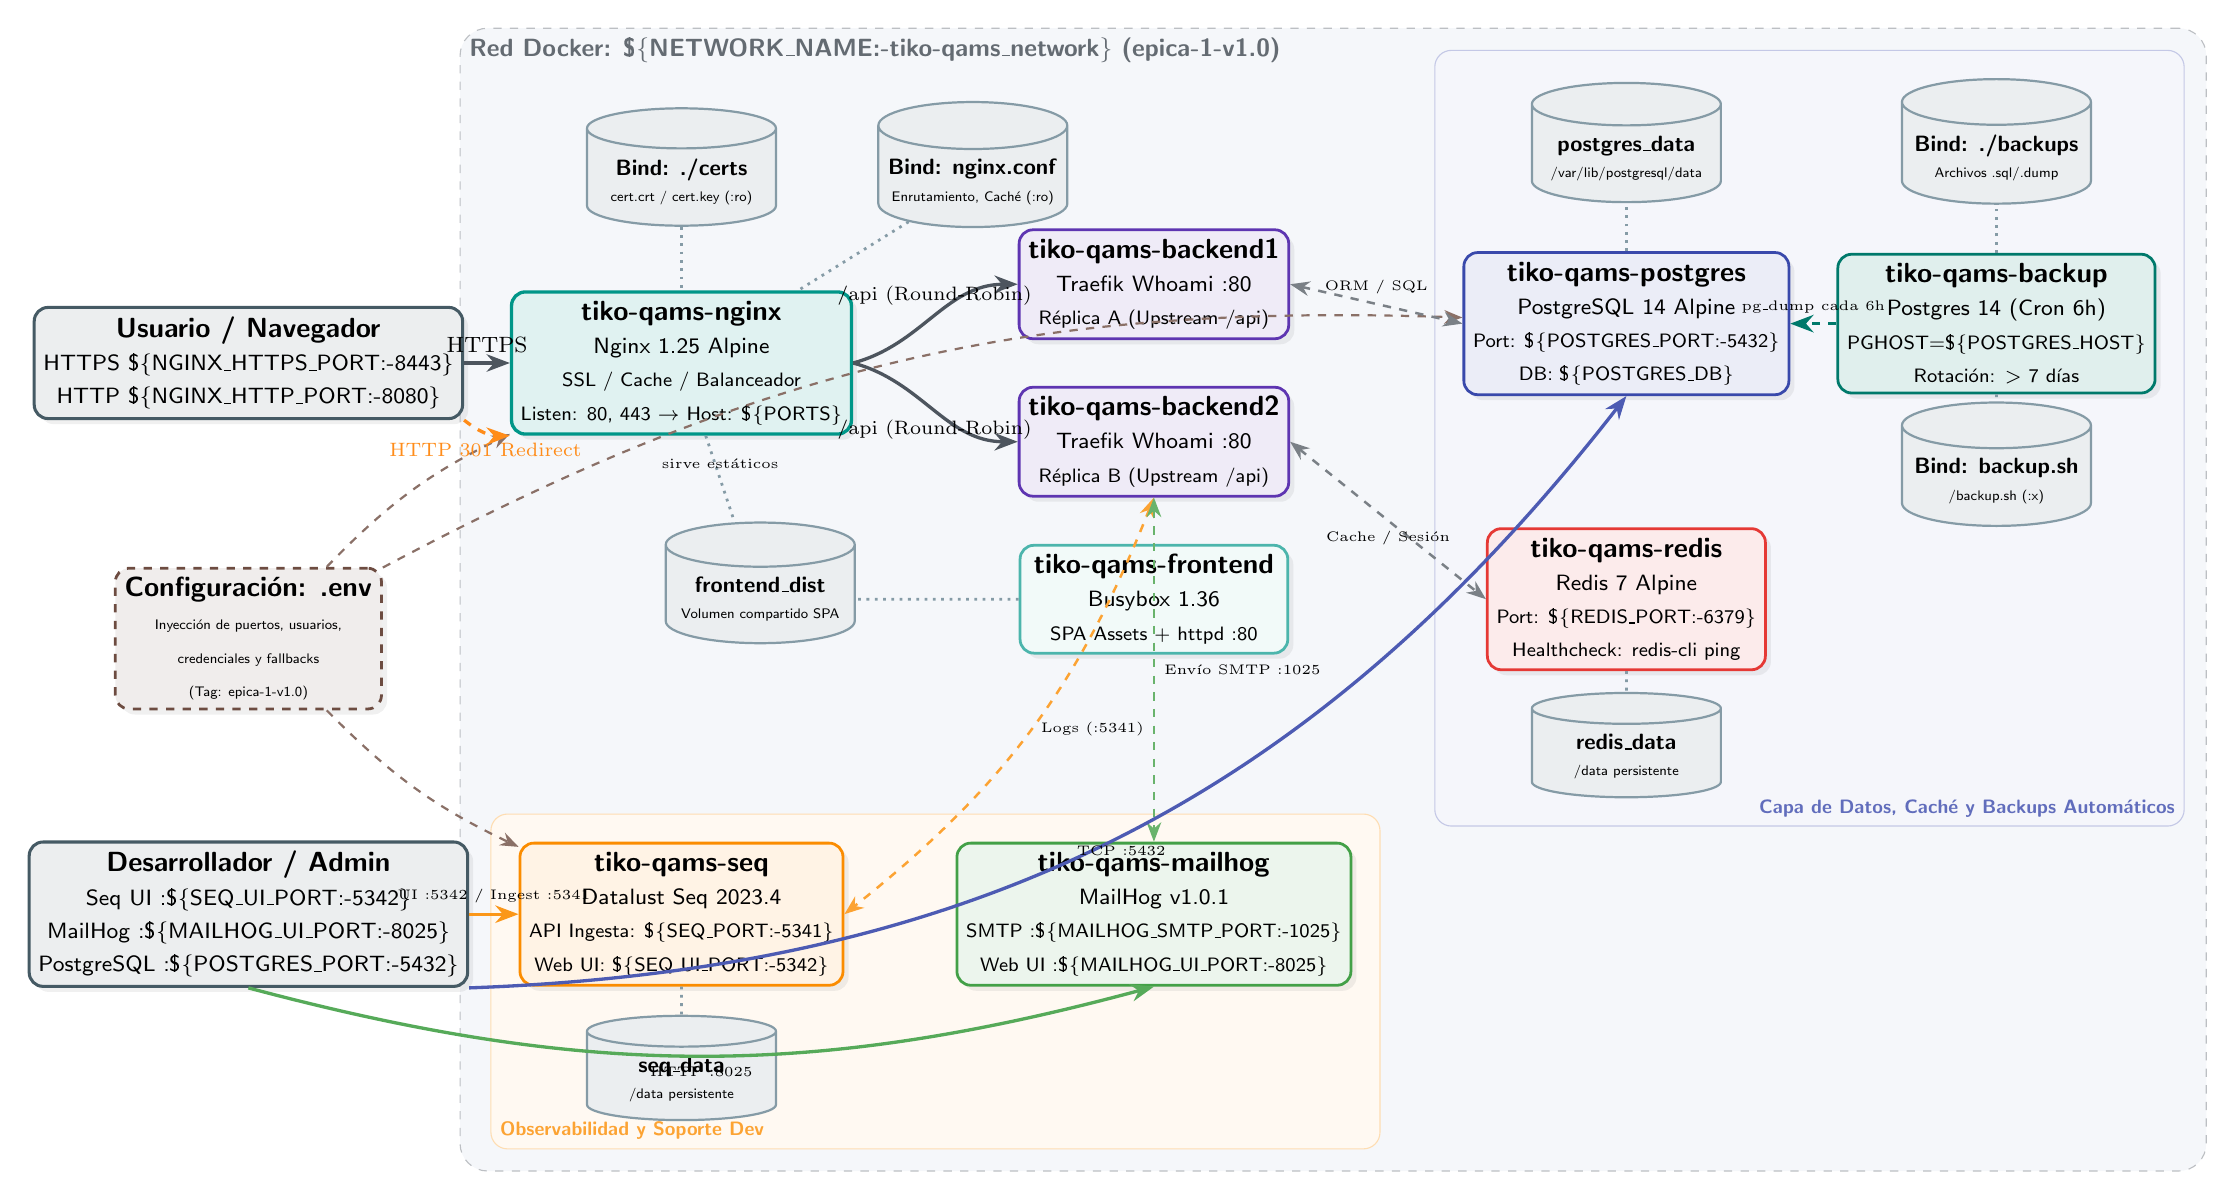
\begin{tikzpicture}[
    font=\sffamily,
    >=Stealth,
    node distance=1.5cm and 1.8cm,
    % Estilos base
    card/.style={
        rectangle,
        rounded corners=5pt,
        draw=colordark!70,
        line width=0.8pt,
        minimum width=3.4cm,
        minimum height=1.3cm,
        align=center,
        fill=white,
        drop shadow={opacity=0.12, shadow xshift=2pt, shadow yshift=-2pt}
    },
    clientnode/.style={
        card,
        draw=colorclient,
        fill=colorclient!10,
        minimum width=3.8cm,
        line width=1.1pt
    },
    gatewaynode/.style={
        card,
        draw=colornginx,
        fill=colornginx!12,
        line width=1.2pt
    },
    backendnode/.style={
        card,
        draw=colorbackend,
        fill=colorbackend!10,
        line width=1pt
    },
    dbnode/.style={
        card,
        draw=colorstorage,
        fill=colorstorage!10,
        line width=1pt
    },
    backupnode/.style={
        card,
        draw=colorbackup,
        fill=colorbackup!12,
        line width=1pt
    },
    redisnode/.style={
        card,
        draw=colorredis,
        fill=colorredis!10,
        line width=1pt
    },
    toolnode/.style={
        card,
        draw=colorseq,
        fill=colorseq!10,
        line width=1pt
    },
    mailnode/.style={
        card,
        draw=colormail,
        fill=colormail!10,
        line width=1pt
    },
    envnode/.style={
        card,
        draw=colorenv,
        fill=colorenv!10,
        dashed,
        minimum width=3.2cm,
        line width=1pt
    },
    volumenode/.style={
        cylinder,
        shape border rotate=90,
        aspect=0.25,
        draw=colorvolume!90,
        fill=colorvolume!15,
        line width=0.8pt,
        minimum width=2.4cm,
        minimum height=1.0cm,
        align=center,
        font=\sffamily\footnotesize
    },
    lineflow/.style={
        ->,
        line width=1.2pt,
        draw=colordark!80
    },
    linedashed/.style={
        <->,
        dashed,
        line width=0.9pt,
        draw=colordark!60
    },
    volumeline/.style={
        -,
        dotted,
        line width=1pt,
        draw=colorvolume!90
    },
    envline/.style={
        ->,
        dashed,
        line width=0.8pt,
        draw=colorenv!80
    }
]

    % ==========================================
    % 1. CLIENTES EXTERNOS / HOST
    % ==========================================
    \node[clientnode] (user) at (0, 7.5) {
        \textbf{Usuario / Navegador}\\
        \footnotesize HTTPS \$\{NGINX\_HTTPS\_PORT:-8443\}\\
        \footnotesize HTTP \$\{NGINX\_HTTP\_PORT:-8080\}
    };

    \node[clientnode] (admin) at (0, 0.5) {
        \textbf{Desarrollador / Admin}\\
        \footnotesize Seq UI :\$\{SEQ\_UI\_PORT:-5342\}\\
        \footnotesize MailHog :\$\{MAILHOG\_UI\_PORT:-8025\}\\
        \footnotesize PostgreSQL :\$\{POSTGRES\_PORT:-5432\}
    };

    % Nodo de Configuración de Variables (.env)
    \node[envnode] (envfile) at (0, 4.0) {
        \textbf{Configuración: .env}\\
        \tiny Inyección de puertos, usuarios,\\
        \tiny credenciales y fallbacks\\
        \tiny (Tag: epica-1-v1.0)
    };

    % ==========================================
    % 2. REVERSE PROXY / INGRESS
    % ==========================================
    \node[gatewaynode] (nginx) at (5.5, 7.5) {
        \textbf{tiko-qams-nginx}\\
        \footnotesize Nginx 1.25 Alpine\\
        \scriptsize SSL / Cache / Balanceador\\
        \scriptsize Listen: 80, 443 $\to$ Host: \$\{PORTS\}
    };

    % Bind mounts de Nginx
    \node[volumenode] (bind_certs) at (5.5, 9.8) {
        \textbf{Bind: ./certs}\\
        \tiny cert.crt / cert.key (:ro)
    };
    \node[volumenode] (bind_nginx) at (9.2, 9.8) {
        \textbf{Bind: nginx.conf}\\
        \tiny Enrutamiento, Caché (:ro)
    };

    % ==========================================
    % 3. CLÚSTER DE SERVICIOS BACKEND & FRONTEND
    % ==========================================
    \node[backendnode] (backend1) at (11.5, 8.5) {
        \textbf{tiko-qams-backend1}\\
        \footnotesize Traefik Whoami :80\\
        \scriptsize Réplica A (Upstream /api)
    };

    \node[backendnode] (backend2) at (11.5, 6.5) {
        \textbf{tiko-qams-backend2}\\
        \footnotesize Traefik Whoami :80\\
        \scriptsize Réplica B (Upstream /api)
    };

    \node[backendnode, draw=colornginx!70, fill=colornginx!5] (frontend) at (11.5, 4.5) {
        \textbf{tiko-qams-frontend}\\
        \footnotesize Busybox 1.36\\
        \scriptsize SPA Assets + httpd :80
    };

    \node[volumenode] (vol_frontend) at (6.5, 4.5) {
        \textbf{frontend\_dist}\\
        \tiny Volumen compartido SPA
    };

    % ==========================================
    % 4. PERSISTENCIA, CACHÉ Y BACKUPS
    % ==========================================
    \node[dbnode] (postgres) at (17.5, 8.0) {
        \textbf{tiko-qams-postgres}\\
        \footnotesize PostgreSQL 14 Alpine\\
        \scriptsize Port: \$\{POSTGRES\_PORT:-5432\}\\
        \scriptsize DB: \$\{POSTGRES\_DB\}
    };

    \node[volumenode] (vol_postgres) at (17.5, 10.1) {
        \textbf{postgres\_data}\\
        \tiny /var/lib/postgresql/data
    };

    \node[backupnode] (backup) at (22.2, 8.0) {
        \textbf{tiko-qams-backup}\\
        \footnotesize Postgres 14 (Cron 6h)\\
        \scriptsize PGHOST=\$\{POSTGRES\_HOST\}\\
        \scriptsize Rotación: $>$ 7 días
    };

    \node[volumenode] (bind_backups) at (22.2, 10.1) {
        \textbf{Bind: ./backups}\\
        \tiny Archivos .sql/.dump
    };

    \node[volumenode] (bind_script) at (22.2, 6.0) {
        \textbf{Bind: backup.sh}\\
        \tiny /backup.sh (:x)
    };

    \node[redisnode] (redis) at (17.5, 4.5) {
        \textbf{tiko-qams-redis}\\
        \footnotesize Redis 7 Alpine\\
        \scriptsize Port: \$\{REDIS\_PORT:-6379\}\\
        \scriptsize Healthcheck: redis-cli ping
    };

    \node[volumenode] (vol_redis) at (17.5, 2.5) {
        \textbf{redis\_data}\\
        \tiny /data persistente
    };

    % ==========================================
    % 5. OBSERVABILIDAD Y HERRAMIENTAS DEV
    % ==========================================
    \node[toolnode] (seq) at (5.5, 0.5) {
        \textbf{tiko-qams-seq}\\
        \footnotesize Datalust Seq 2023.4\\
        \scriptsize API Ingesta: \$\{SEQ\_PORT:-5341\}\\
        \scriptsize Web UI: \$\{SEQ\_UI\_PORT:-5342\}
    };

    \node[volumenode] (vol_seq) at (5.5, -1.6) {
        \textbf{seq\_data}\\
        \tiny /data persistente
    };

    \node[mailnode] (mailhog) at (11.5, 0.5) {
        \textbf{tiko-qams-mailhog}\\
        \footnotesize MailHog v1.0.1\\
        \scriptsize SMTP :\$\{MAILHOG\_SMTP\_PORT:-1025\}\\
        \scriptsize Web UI :\$\{MAILHOG\_UI\_PORT:-8025\}
    };

    % ==========================================
    % CONEXIONES / FLUJOS DE DATOS
    % ==========================================
    % Inyección de Configuración (.env)
    \draw[envline] (envfile) to[bend left=10] (nginx);
    \draw[envline] (envfile) to[bend right=10] (seq);
    \draw[envline] (envfile) to[bend left=15] (postgres);

    % Cliente -> Nginx
    \draw[lineflow] (user) -- node[above, font=\footnotesize] {HTTPS} (nginx);
    \draw[lineflow, dashed, draw=orange!90] (user.south east) to[bend right=20] 
        node[below, font=\scriptsize, text=orange!90] {HTTP 301 Redirect} (nginx.south west);

    % Nginx Binds & Volumes
    \draw[volumeline] (bind_certs) -- (nginx);
    \draw[volumeline] (bind_nginx) -- (nginx);
    \draw[volumeline] (nginx) -- node[above, font=\tiny] {sirve estáticos} (vol_frontend);
    \draw[volumeline] (frontend) -- (vol_frontend);

    % Nginx -> Backends (Load Balancing)
    \draw[lineflow] (nginx.east) to[out=15, in=180] 
        node[above, font=\scriptsize] {/api (Round-Robin)} (backend1.west);
    \draw[lineflow] (nginx.east) to[out=-15, in=180] 
        node[below, font=\scriptsize] {/api (Round-Robin)} (backend2.west);

    % Backends -> PostgreSQL & Redis
    \draw[linedashed] (backend1.east) -- node[above, font=\tiny] {ORM / SQL} (postgres.west);
    \draw[linedashed] (backend2.east) -- node[below, font=\tiny] {Cache / Sesión} (redis.west);

    % Postgres Volumes & Backup Service
    \draw[volumeline] (postgres) -- (vol_postgres);
    \draw[lineflow, draw=colorbackup, dashed] (backup.west) -- node[above, font=\tiny] {pg\_dump cada 6h} (postgres.east);
    \draw[volumeline] (backup) -- (bind_backups);
    \draw[volumeline] (backup) -- (bind_script);

    % Redis Volume
    \draw[volumeline] (redis) -- (vol_redis);

    % Backends -> Seq & Mailhog
    \draw[linedashed, draw=colorseq!80] (backend2.south) to[bend left=15] 
        node[right, font=\tiny] {Logs (:5341)} (seq.east);
    \draw[linedashed, draw=colormail!80] (backend2.south) -- 
        node[right, font=\tiny] {Envío SMTP :1025} (mailhog.north);

    % Admin / Dev Direct Access
    \draw[lineflow, draw=colorseq!90] (admin) -- node[above, font=\tiny] {UI :5342 / Ingest :5341} (seq);
    \draw[lineflow, draw=colormail!90] (admin.south) to[bend right=15] 
        node[below, font=\tiny] {HTTP :8025} (mailhog.south);
    \draw[lineflow, draw=colorstorage!90] (admin.south east) to[bend right=25] 
        node[below, font=\tiny] {TCP :5432} (postgres.south);

    % Seq Volume
    \draw[volumeline] (seq) -- (vol_seq);

    % ==========================================
    % FONDOS Y CONTENEDORES (GRUPOS)
    % ==========================================
    \begin{scope}[on background layer]
        % Red docker bridge
        \node[
            fill=colorbgnet,
            draw=colordark!30,
            dashed,
            rounded corners=10pt,
            fit=(nginx) (backend1) (backend2) (frontend) (postgres) (redis) (backup) (seq) (mailhog) (vol_frontend) (bind_certs) (vol_postgres) (vol_redis) (vol_seq) (bind_backups) (bind_script),
            inner sep=18pt
        ] (docker_network) {};
        \node[anchor=north west, font=\sffamily\bfseries\small, text=colordark!70] 
            at (docker_network.north west) {Red Docker: \$\{NETWORK\_NAME:-tiko-qams\_network\} (epica-1-v1.0)};

        % Agrupación Data & Backup Layer
        \node[
            fill=colorstorage!5,
            draw=colorstorage!30,
            rounded corners=6pt,
            fit=(postgres) (redis) (backup) (vol_postgres) (vol_redis) (bind_backups) (bind_script),
            inner sep=10pt
        ] (group_data) {};
        \node[anchor=south east, font=\sffamily\scriptsize\bfseries, text=colorstorage!80] 
            at (group_data.south east) {Capa de Datos, Caché y Backups Automáticos};

        % Agrupación Observabilidad
        \node[
            fill=colorseq!5,
            draw=colorseq!30,
            rounded corners=6pt,
            fit=(seq) (mailhog) (vol_seq),
            inner sep=10pt
        ] (group_obs) {};
        \node[anchor=south west, font=\sffamily\scriptsize\bfseries, text=colorseq!80] 
            at (group_obs.south west) {Observabilidad y Soporte Dev};
    \end{scope}

\end{tikzpicture}
\end{document}
